\documentclass[12pt, titlepage]{article}
\usepackage{graphicx}
\usepackage{amsmath}
\usepackage{esint}
\usepackage{tcolorbox}
\usepackage{parskip}
\usepackage[]{fancyhdr}
\usepackage{pgfplots}
\usepackage{mdframed}
\usepackage{multicol}
\pgfplotsset{compat=1.18}
\setlength{\headheight}{15pt}
\tcbuselibrary{breakable}

\title{Magnetic Fields and Electromagnetism}
\author{Matthew Pan}
\date{April 2025}

\newtcolorbox{Problem}{colback=blue!5!white,colframe=blue!50!black,title=Problem, breakable=true}

\begin{document}

\pagestyle{fancy}

\fancyhead{}
\fancyhead[L]{Pan}
\fancyhead[R]{\thepage}

\maketitle

\section*{12.1 Magnetic Fields}

A magnetic field is a vector field that describes the magnetic force exerted on moving charges, electric currents, or magnetic materials. On a microscopic level, magnetic dipoles are created by the circular or rotational motion of electric charges, such as electrons. Since magnetic fields are created by magnetic dipoles, which always have a north and a south pole, magnetic field lines always form a closed loop: north to south outside a magnet and south to north inside a magnet. Magnetic fields can never occur as a monopole, meaning the north and south poles of a magnet cannot be separated.

Because magnetic poles always occur as dipoles, the net magnetic field through any closed surface will always be zero. This is Maxwell's second equation.
\begin{equation*}
    \oiint B \cdot dA = 0
\end{equation*}

Magnetic permeability describes a substance's ability to form internal magnetic fields, represented by $\mu$. A material's relative permeability is its actual permeability divided by the permeability of free space.
\begin{equation*}
    \mu_r = \frac{\mu}{\mu_0}
\end{equation*}

The E\&M course teaches three types of magnetism:
\begin{enumerate}
    \item \textbf{Ferromagnetism} - Found in permanent magnets - the magnetic moments continue to be aligned after exposure to a magnetic field, producing its own field. 
    \item \textbf{Paramagnetism} - A weak alignment of magnetic moments within a material when exposed to an external magnetic field. the moments become disaligned when the field is removed. $\mu_r$ is close to 1.
    \item \textbf{Diamagnetism} - A weak alignment of magnetic moments within a material when exposed to an external magnetic field. The magnetic moments align in the opposite direction as the external field. The moments become disaligned when the field is removed. This property is present in all materials, but is usually neglible unless no other magnetic effects are present. $\mu_r$ is close to 1.
\end{enumerate}

\section*{12.2 Magnetism and Moving Charges}
\subsection*{Magnetic Fields Produced by Charges}

Moving charge carriers produce magnetic fields. The magnitude and direction of a magnetic field is defined by the Biot-Savart Law:
\begin{equation*}
    d\vec{B} = \frac{\mu_0}{4\pi}\frac{Id\vec{l}\times\hat{r}}{r^2}
\end{equation*}

In this section, we are most concerned about finding the direction of the magnetic field. We will find the magnitude in later sections.

Notice the cross product in the Biot-Savart law---we can find this using the right hand rule. When finding the cross product $\vec{C}=\vec{A}\times\vec{B}$, your pointer finger represents $\vec{A}$, your middle finger represents $\vec{B}$, and your thumb represents $\vec{C}$. Always keep your thumb orthogonal to your pointer and middle fingers.

We can apply a simplified version of the Biot-Savart law to find the \textbf{direction of a magnetic field only}.
\begin{equation*}
    B=v\times\hat{r}
\end{equation*}
Where
\begin{itemize}
    \item \textbf{$B$} is the direction of the magnetic field
    \item \textbf{$v$} is the direction that the charged particle is traveling in 
    \item \textbf{$\hat{r}$} points away from moving charge towards where you are measuring the magnetic field
\end{itemize}

\begin{center}
    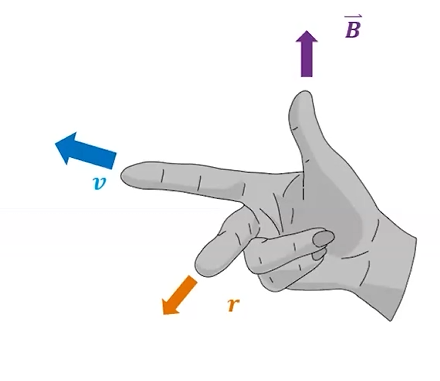
\includegraphics[height=4cm]{media/rh1.png}
\end{center}

When we apply this to many points around the moving charge, we find that the magnetic field forms a concentric circles around the charge, leading us to the next right hand rule.

When making a ``thumbs up'' hand gesture, the thumb points in the direction of the current, the the other fingers curl in the direction that the field circles in around the moving charged object.
\begin{center}
    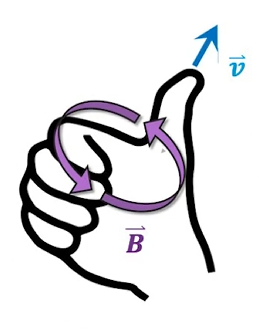
\includegraphics[height=4cm]{media/rh2_2.png}
    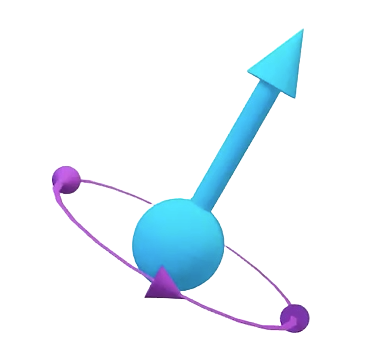
\includegraphics[height=4cm]{media/rh2.png}
\end{center}

\subsection*{Moving Charges in Magentic Fields}

A charged particle moving in a magnetic field experiences a force determined by the Lorentz force equation:

\begin{equation*}
    \vec{F_B} = q(\vec{v}\times\vec{B})
\end{equation*}
\begin{Problem}
    A particle is traveling with a constant velocity to the right, while a uniform magnetic field is directed out of the page. Describe the motion of the particle.
    \tcblower
    \textit{Solution. } We can apply the right hand rule with the equation above. At the instant described in the scenario, the force is directed downwards. Since the force will always be orthogonal to the velocity and magnetic field vectors, we can say that the force is centripetal, and the particle moves in circular motion.
    
    Note that the magnetic field cannot speed or slow the particle down and does no work on the object. The radius of the circle can be calculated by setting $\vec{F}_B$ to the centripetal force equation, $\frac{mv^2}{r}$
\end{Problem}

Let's take a look at another scenario, this time also combining an electric field: 

Consider a positively charged particle moving rightward with a constant velocity through a space where there is an electric field going up and a magnetic field out of the page. The particle will experience both an electric and magnetic force. Because the particle is positively charged, the electric force acts upwards. Using the right hand rule, we find that the magnetic field forces the particle down. 

We can find the velocity that will cause the particle to move in a straight line by setting $\vec{F}_B$ and $\vec{F}_E$ equal to each other:
\begin{align*}
    \vec{F}_B &= \vec{F}_E \\
    qE &= qvB \\
    v &= \frac{E}{B}
\end{align*}
If the particle is slower than this velocity, the electric force will be greater than the magnetic force.
\subsection*{The Hall Effect}

Consider the following circuit:
\begin{center}
    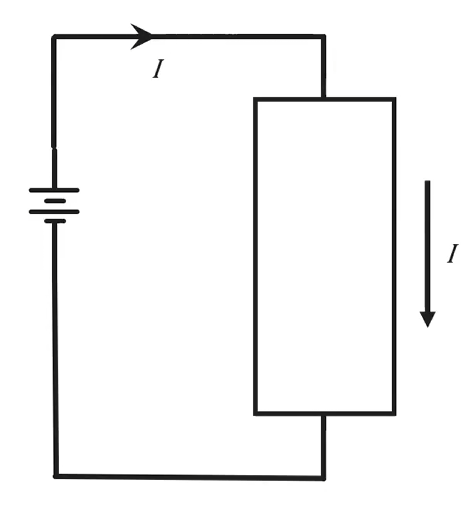
\includegraphics[height=4cm]{media/halleffect.png}
\end{center}

What would be the effect of an external magnetic field, directed out of the page, on the movement of electrons?

As the electrons flow up through the magnetic field, they experience a magnetic force directed leftward, causing electrons to accumulate on the left side of the wire. This causes an opposing electric force that balances the magnetic force and an electric field directed leftward. We can measure a difference in electric potential, called the Hall voltage, to determine the strength of the magnetic field.

\section*{12.3 Magnetic Fields of Current-Carrying Wires and the Biot-Savart Law}

\subsection*{Magnetic Forces on a Current Carrying Wire}
In this subsection, we are interested in determining how much force is applied to a current carrying wire in a magnetic field, as opposed to a force applied to a single charge carrier in a magnetic field. The Lorentz force equation for this is very similar to a previous equation.
\begin{equation*}
    \vec{F_B} = q(\vec{v}\times\vec{B}) \quad \textrm{vs.} \quad \vec{F_B} = \int I \, d\vec{l} \times \vec{B}
\end{equation*}
Where
\begin{itemize}
    \item $\vec{F_B}$ is the total force on the wire due to a magnetic field $\vec{B}$
    \item $I$ is the magnitude of current in the wire
    \item $d\vec{l}$ is an infinitesimally small section of wire, which always points in the direction of conventional current
    \item $\vec{B}$ is the magnetic field at the location $d\vec{l}$
\end{itemize}

\subsection*{The Biot-Savart Law}

In a previous section, we determined the direction of a magnetic field caused by a current carrying wire. Now, we need to know how to find the magnitude of that magnetic field. Generally, the Biot Savart law should only be used when arcs of current are present. Ampere's law should be used in other cases.
\begin{equation*}
    d\vec{B} = \frac{\mu_0}{4\pi}\frac{Id\vec{l}\times\hat{r}}{r^2}
\end{equation*}
\subsubsection*{Infinitely Long Wire}
\begin{center}
    \includegraphics*[height=4cm]{media/longwire.png}
\end{center}
In this example, we need to sum the magnetic fields that each small segment of wire, $d\vec{l}$ is producing. As we get farther from the wire, the magnetic field gets weaker, so the contribution of each small section of wire decreases as we approach negative or positive infinity. \textbf{College Board does not require you to know the following derivation. Skip it if you want.}

Setting up the integral for the magnetic field at point P:
\begin{equation*}
    \vec{B}_P = \frac{\mu_0}{4\pi} \int \frac{Id\vec{l}\times\hat{r}}{r^2}
\end{equation*}
We only need the magnitude of magnetic field:
\begin{equation*}
    B_P = \frac{\mu_0}{4\pi} \int \frac{Idl\sin(\theta)}{r^2}
\end{equation*}
$r$, the distance from point $P$ to a section of wire $dl$ can be represented as $\sqrt{r_{\perp}^2+x^2}$. We can also make the substitution $dl=dx$ because they lie in the same direction. $\sin(\theta)$ can be substituted for $\frac{x}{\sqrt{r_{\perp}^2+x^2}}$. The wire is infinitely long, so we will be integrating from $x=-\infty$ to $x=+\infty$. Since $I$ is constant, we can remove it from the integral. For simplicity, we will now define $d=r_{\perp}$. The following integral can be solved with trig substitution.
\begin{equation*}
    |\vec{B}_P| = \frac{\mu_0I}{4\pi} \int_{-\infty}^{+\infty} \frac{d \, dx}{(x^2+d^2)^{\frac{3}{2}}}
\end{equation*}
\begin{equation*}
    \textrm{let} \ x=d\cot(\theta)\textrm{,} \ dx = -d\csc^2(\theta) \, d\theta\textrm{, and} \ \sqrt{d^2+x^2} = d\csc(\theta)
\end{equation*}
Substituting:
\begin{align*}
    &\int_{\pi}^{0} \frac{-d^2 \csc^2(\theta)}{d^3\csc^3(\theta)} d\theta \\
    =&-\frac{1}{d} \int_{\pi}^{0} \sin(\theta) d\theta \\
    =& \left.{\left [\frac{\cos(\theta)}{d}\right]}\right |_{\; \pi}^{\; 0}
    =\frac{2}{d}
\end{align*}
Thus:
\begin{equation*}
    \boxed{|\vec{B}_P|=\frac{\mu_0I}{2\pi d}}
\end{equation*}

\subsubsection*{Loop of Current}
Applying the Biot-Savart law to arcs of current when measuring the magnetic field from the center of the arc is more straightforward, thankfully, since all $dl$ is equidistant from the center ($r$ is a constant and can be pulled out of the integral) and $d\vec{l} \times \hat{r}$ = $dl$ ($d\vec{l}$ and $\hat{r}$ are orthogonal).

Considering a loop of current: 
\begin{center}
    \includegraphics*[height=4cm]{media/loop.png}
\end{center}
\begin{align*}
    |\vec{B}_P| =& \frac{\mu_0}{4\pi} \int \frac{Id\vec{l}\times\hat{r}}{r^2} \\
    =& \frac{\mu_0I}{4 \pi R^2} \int dl \\
    =& \frac{\mu_0I}{4 \pi R^2} \cdot 2\pi R = \boxed{\frac{\mu_0I}{2R}}
\end{align*}
When we are integrating $dl$, we are really just adding up all of the small lengths of wire that compose the loop --- the circumfrence of the circle.

\subsubsection*{Arcs of Current}
\begin{center}
    \includegraphics*[height=4cm]{media/bentloop.png}
\end{center}
\begin{align*}
    |\vec{B}_P| =& \frac{\mu_0}{4\pi} \int \frac{Id\vec{l}\times\hat{r}}{r^2} \\
    =& \frac{\mu_0I}{4 \pi R^2} \int_{0}^{R \theta} dl \\
    =& \frac{\mu_0I}{4 \pi R^2} \cdot R\theta = \boxed{\frac{\mu_0 \theta I}{4 \pi R}}
\end{align*}
This derivation appears to only find the magnetic field contribution for the arc. What about the straight sections?

Notice that for all $d\vec{l}$, $\hat{r}$, the unit vector pointing from $d\vec{l}$ to the center, is pointed in the same direction --- the angle between $d\vec{l}$ and $\hat{r}$ is 0. Because the cross product of two vectors pointed in the same direction is always 0, there is no magnetic field contribution from the straight sections of the wire.

\subsubsection*{Axis of a Loop of Current}

\begin{center}
    \includegraphics*[height=4cm]{media/axis.png}
\end{center}

\begin{align*}
    |\vec{B}_P| =& \frac{\mu_0}{4\pi} \int \frac{Id\vec{l}\times\hat{r}}{r^2} \\
    =& \frac{\mu_0I}{4 \pi r^2} \cdot \cos(\beta)\int dl \\
    =& \frac{\mu_0I}{4 \pi (R^2+h^2)} \cdot \frac{R}{\sqrt{R^2+h^2}} \cdot 2 \pi R \\
    =& \boxed{\frac{\mu_0 IR^2}{2(R^2+h^2)^\frac{3}{2}}}
\end{align*}

Each $d\vec{B}$ vector is pointing out from the axis at an angle $\beta$. We can take the cosine of $d\vec{B}$ to get $d\vec{B}_x$, the x component of the magnetic field caused by $d\vec{l}$, using the following subsitutions:
\begin{itemize}
    \item $r^2=R^2+h^2$ --- the distance between a point on the loop and the point we are calculating the magnetic field from.
    \item $\cos (\beta) = \frac{R}{\sqrt{R^2+h^2}}$ --- The angle $\beta$ is equal to the angle formed by $R$ and $r$ 
\end{itemize}

\section*{12.4 Ampere's Law}

Ampere's Law relates the magnetic field created in space to the current enclosed by an imagnary closed path called an Amperian loop. Ampere's Law with Maxwell's extension is called Maxwell's Fourth Equation.
\begin{equation*}
    \oint \vec{B} \cdot d\vec{l}= \mu_0I_{enc} + \mu_0\epsilon_0\frac{d\phi_E}{dt}
\end{equation*}
\begin{minipage}{\textwidth}
Where
\begin{itemize}
    \item $\vec{B} \cdot d\vec{l}$ is the dot product of the magnetic field and a small section of the Amperian loop.
    \item $\mu_0I_{enc}$ is the product of the permeability of free space and the current enclosed by the Amperian loop.
    \item $\mu_0\epsilon_0\frac{d\phi_E}{dt}$ is Maxwell's extension to Ampere's law. Maxwell's extension is not on the formula sheet, nor is applying it tested, but \textit{you should know that a changing electric field generates a magnetic field.}
\end{itemize}
\end{minipage}

When applying Ampere's Law to AP Physics C, we can make a few simplifications. These also provide the guidelines for drawing an Amperian loop:
\begin{itemize}
    \item We can simplify the dot product to only find the magnitude
    \item The magnetic field should always be constant at the loop so that it can be pulled out of the integral
    \item The magnetic field should always point in the same direction as the Amperian loop so that $\cos\theta=1$
\end{itemize}
After this, we are left with 
\begin{equation*}
    B \oint dl = \mu_0I_{enc}
\end{equation*}
$\oint dl$ will become the length of the path (usually the perimeter). Let's take a look at a few cases.

\subsubsection*{Infinitely Long Wire}

\begin{center}
    \includegraphics*[height=6cm]{media/amperelongwire.png}
\end{center}
\begin{align*}
    \oint \vec{B} \cdot d\vec{l} &= \mu_0I_{enc} \\
    B(2\pi R) &= \mu_0 I \\
    B &= \boxed{\frac{\mu_0 I}{2\pi R}}
\end{align*}
We get the same answer as using the Biot-Savart law with a quarter of the work.

\subsubsection*{Coaxial Wire}

\begin{center}
    \includegraphics*[height=4cm]{media/coaxial.png}
\end{center}
We can define four regions to apply Ampere's law:
\begin{multicols}{2}
    \begin{itemize}
        \item $r<a$ 
        \item $a<r<b$ 
        \item $b<r<c$ 
        \item $r>c$ 
    \end{itemize}
\end{multicols}
\textbf{When $r<a$:}
Since our Amperian loop lies within the inner conductor and does not enclose the full current $I$, we must use the current density to calculate the portion of current enclosed.
\begin{equation*}
    J=\frac{I}{A}=\frac{I}{\pi a^2}
\end{equation*}
\begin{align*}
    \oint \vec{B} \cdot d\vec{l} &= \mu_0I_{enc} \\
    B(2\pi r) &= \mu_0 JA_{enc} \\
    B &= \frac{\mu_0}{2 \pi r} \frac{I\pi r^2}{\pi a^2} \\
    &= \boxed{\frac{\mu_0Ir}{2 \pi a^2}}
\end{align*}

\textbf{When $a<r<b$:} We enclose current $I$ in a radius $r$.
\begin{align*}
    \oint \vec{B} \cdot d\vec{l} &= \mu_0I_{enc} \\
    B(2\pi r) &= \mu_0 I \\
    B &= \boxed{\frac{\mu_0 I}{2\pi r}}
\end{align*}

\textbf{When $b<r<c$:} Again, the Amperian loop lies within a conductor and does not enclose the full current. We must use current density. Note that the current is going in the negative direction, so we need to subract it from the current from the inside wire.
\begin{equation*}
    J=\frac{I}{A}=\frac{I}{\pi(c^2-b^2)}
\end{equation*}
\begin{align*}
    \oint \vec{B} \cdot d\vec{l} &= \mu_0I_{enc} \\
    B(2\pi r) &= \mu_0 (I-JA_{enc}) \\
    B &= \frac{\mu_0}{2 \pi r} (I- \frac{I\pi (r^2-b^2)}{\pi (c^2-b^2)}) \\
    &= \boxed{\frac{\mu_0I}{2 \pi r}(1-\frac{r^2-b^2}{c^2-b^2})}
\end{align*}
\textbf{When $r>c$:} We enclose zero current, so there is no magnetic field outside of the cable.

\subsubsection*{Solenoids}

A solenoid is a coil of wire In an ideal solenoid, there will be no edge effects, no resistance in the wires, the wire will be coiled with no gaps, and the magnetic field outside the coils of a solenoid will be zero. 

In this case, we need to draw an Amperian loop shaped like a rectangle:
\begin{center}
    \includegraphics*[height=4cm]{media/solenoid.png}
\end{center}
The magnetic field contribution of the left and right edges are zero, since the magnetic field and the edges are orthogonal. The magnetic field outside of the solenoid is also zero, leaving the inside portion. The current enclosed by the Amperian loop is the current going through the loops times the number of loops, $N$. The number of loops per unit length is $n$
\begin{align*}
    \oint \vec{B} \cdot d\vec{l} &= \mu_0I_{enc} \\
    B(w) &= \mu_0NI \\
    B &= \boxed{\mu_0nI}
\end{align*}
\end{document}